\documentclass[a4paper, 11pt, table]{article}

\usepackage[utf8]{inputenc}
\usepackage[english]{babel}
\usepackage[table]{xcolor}
\usepackage{graphicx}
\usepackage{tikz}
\usetikzlibrary{calc}
\usepackage{float}
\usepackage{pifont,mdframed}
\usepackage{subfig}
\usepackage{amsmath}
\usepackage{siunitx}
\sisetup{
    group-digits=true,
    group-separator={\,},
}
\usepackage{caption}
\usepackage{pifont}
\usepackage{footnote}
\makesavenoteenv{tabular}
\usepackage{pgfplots}
\usetikzlibrary{pgfplots.groupplots}
\usetikzlibrary{matrix}
\usepackage{booktabs}
\usepackage{csquotes}
\usepackage{afterpage}
\usepackage{pdflscape}

\usepackage[
backend=biber
]{biblatex}
\addbibresource{references.bib}

\definecolor{Gray}{gray}{0.9}
\definecolor{LabelColor}{gray}{0.0}
\definecolor{clno}{RGB}{212, 59, 59}
\definecolor{clyes}{RGB}{12, 150, 12}
\definecolor{linux}{RGB}{255, 186, 249}
\definecolor{windows}{RGB}{186,215, 255}
\definecolor{macos}{gray}{0.9}  
\newcommand{\cmark}{\ding{51}}%
\newcommand{\xmark}{\ding{55}}%
\newcommand{\ymark}{\textcolor{clyes}{\cmark}}%
\newcommand{\nmark}{\textcolor{clno}{\xmark}}%

% Roman numerals
\newcommand{\rom}[1]{\uppercase\expandafter{\romannumeral #1\relax}}

% plots
% https://www.sharelatex.com/learn/Pgfplots_package
\pgfplotsset{width=10cm,compat=1.9}
%\usepgfplotslibrary{external} 
%\tikzexternalize

% short for multicolumn-centered
\newcommand{\mcc}[1]{\multicolumn{1}{c}{#1}}

% http://tex.stackexchange.com/questions/2441/how-to-add-a-forced-line-break-inside-a-table-cell
\newcommand{\specialcell}[2][c]{%
  \begin{tabular}[#1]{@{}c@{}}#2\end{tabular}}

\graphicspath{ {img/} }

% warning environment
% It should not be included in final report
% http://tex.stackexchange.com/questions/8689/how-to-create-a-warning-box-like-this-see-the-figure-to-get-the-idea
\newenvironment{warning}
  {\par\begin{mdframed}[linewidth=2pt,linecolor=red]%
    \begin{list}{}{\leftmargin=1cm
                   \labelwidth=\leftmargin}\item[\Large\ding{43}]}
  {\end{list}\end{mdframed}\par}

\title{Convolutional neural networks for classification of transmission electron microscopy imagery}

\author{Sergii Gryshkevych}
\date{\today}

\begin{document}

\maketitle

\tableofcontents

\begin{abstract}
An abstract.
\end{abstract}

\section{Introduction}



\subsection{Project Goals}

The goal of this project is to study and evaluate the suitability of applying CNN method for automatic classification of electron microscopy (EM) images. Different models based on CNN are compared to and benchmarked against SVM classifier. 


\section{Background}

One of Vironova's electron microscopy (EM) services is to classify types of liposomes. This includes two tasks:



\subsection{Problem description}

A liposome is a sperical vesicle having at least one lipid bilayer~\cite{betageri1993liposome}. Liposomes were first described in 1964 by A.D. Bangham and R.W. Thorne and G. Weissman suggested the name "liposome"~\cite{betageri1993liposome}. Liposomes can be classified into different types according to numerous features such as but not limited to size, number of lamellae, composition, shape, production method, etc. The classification of liposomes was first presented at a meeting of New York Academy of Science~\cite{liposomes1978}. This project focuses on classification of liposomes according to the number of lamellae and response to drugs encapsulation.

\subsubsection{Lamellarity}
\label{sec:lamellarity}

The term lamellarity refers to the number of lamellae. Lamella, in cell biology, is used to describe numerous plate or disc-like structures at both a tissue and cellular level~\cite{cammack2006oxford}. According to number of lamellae liposomes can be unilamellar (single lamella) and multilamellar (multiple lamellae). In addition uncertain class is introduced because in some cases it is almost impossible to be certain about lamellarity class. For example liposomes can overlap each other. Another issue to keep in mind is that samples are usually delivered frozen, so liposomes may be partly covered with pieces of ice that result in large black bulbs on EM images. Figure~\ref{fig:lamellarity_problem} illustrates examples of liposomes from each class.

\begin{figure}[H]
\centering
\begin{tabular}{ccc}
	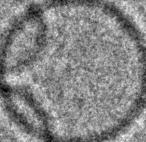
\includegraphics[height=2cm, keepaspectratio]{problem_description/lamellarity/uni} & 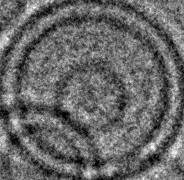
\includegraphics[height=2cm, keepaspectratio]{problem_description/lamellarity/multi} & 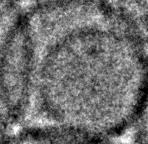
\includegraphics[height=2cm, keepaspectratio]{problem_description/lamellarity/uncertain} \\
	Unilamellar & Multiilamellar & Uncertain \\[6pt]
\end{tabular}
\caption{Lamellarity problem, 3 classes}
\label{fig:lamellarity_problem}
\end{figure}

Table~\ref{table:lamellarity_data_set} present lamellarity problem data set which contains $\num{14169}$ EM images.

\begin{center}
\captionof{table}{Lamellarity problem}
\label{table:lamellarity_data_set}
\begin{tabular}{lrr}
\toprule
Unilamellar & \num{12368} & 87.29\% \\ 
Multilamellar & \num{1717} & 12,12\% \\ 
Uncertain & \num{84} & 0,59\% \\ 
\end{tabular} 
\end{center}


\subsubsection{Encapsulation}
\label{sec:encapsulation}

Liposomes can be used as vehicles for drug delivering throughout various destinations in the human body~\cite{betageri1993liposome}. A crucial part of testing this approach is to measure how many liposomes responded to drugs encapsulation and can carry them further. In encapsulation problem liposomes are classified between the following types: full, i.e. liposomes that received  drug substance, empty, i.e. liposomes that remained empty after encapsulation attempt. As in lamellarity problem uncertain class is introduced with the same motivation. Figure~\ref{fig:encapsulation_problem} illustrates different classes of encapsulation problem. Table~\ref{table:encapsulation_dataset} present encapsulation problem data set which contains $\num{24918}$ EM images.

\begin{figure}[H]
\centering
\begin{tabular}{ccc}
	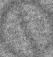
\includegraphics[height=2cm, keepaspectratio]{problem_description/packiging/full} & 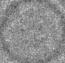
\includegraphics[height=2cm, keepaspectratio]{problem_description/packiging/empty} & 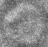
\includegraphics[height=2cm, keepaspectratio]{problem_description/packiging/uncertain} \\
	Full & Empty & Uncertain \\[6pt]
\end{tabular}
\caption{Encapsulation problem, 3 classes}
\label{fig:encapsulation_problem}
\end{figure}


\begin{center}
\captionof{table}{Encapsulation problem}
\label{table:encapsulation_dataset}
\begin{tabular}{lrr}
\toprule
Full & \num{24255} & 97.34\% \\ 
Uncertain & \num{502} & 2.01\% \\ 
Empty & \num{161} & 0.65\% \\ 
\end{tabular} 
\end{center}

\section{The data}
\label{sec:dataset}
The data for this project is provided by Vironova AB. The data consists of two data sets corresponding to lamellarity and inccpsulation problems. Both data sets contain grayscale EM images of particles and a number of computed image features.

Each image depict exactly one liposome. All images are padded 50 pixels in each direction. Effect of particle surrounding on classifier performance is described later in this report. Corresponding particle masks are also provided. All images have different size. Figure~\ref{fig:img_size_scatter_plot} shows scatter plots where axes coordinates correspond to image width and height in pixels. Figure~\ref{fig:img_size_per_class} demonstrates image size distribution inside each class. 

\begin{figure}[H]
\centering
\begin{tabular}{cc}
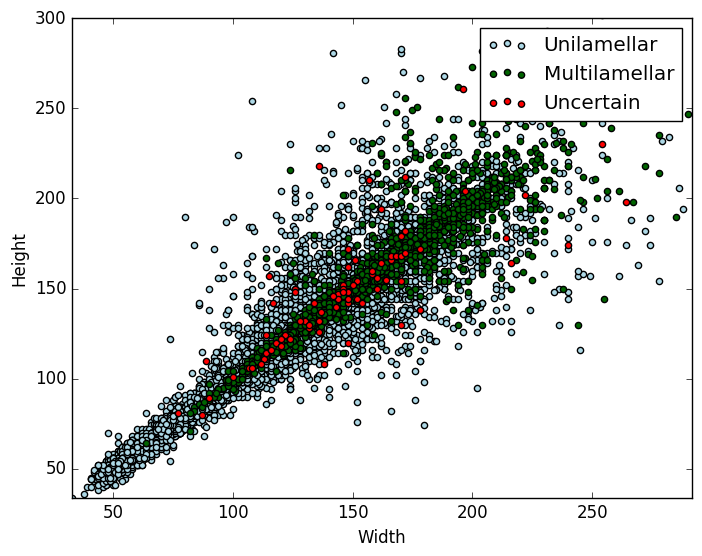
\includegraphics[scale=0.32]{img_size/lamellarity/scatter_plot_width_height.png} & 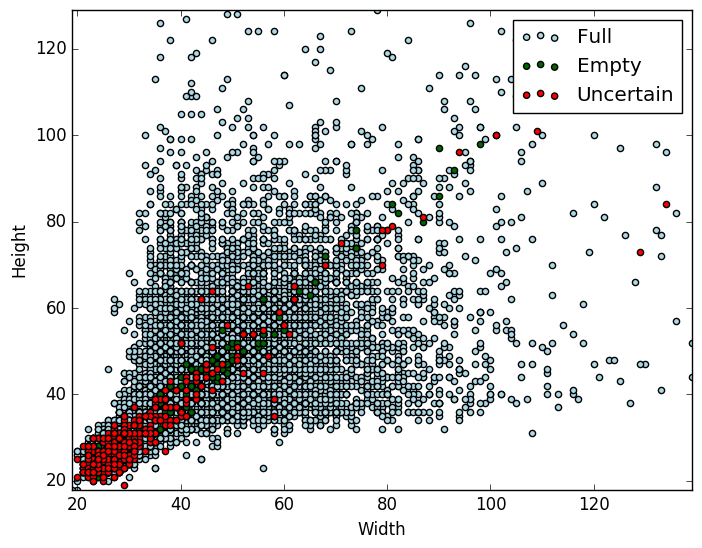
\includegraphics[scale=0.32]{img_size/encapsulation/scatter_plot_width_height.png}
\end{tabular}
\caption{Scatter plots of images sizes (best viewed in color): lamellarity data set to the left hand side, encapsulation --- to the rights hand side. Width and height units are pixels.}
\label{fig:img_size_scatter_plot}
\end{figure}

%\pagebreak
Both data sets contain following features:
\begin{itemize}
\item \textbf{Maximum width} in nanometres. If particle is an ellipse then it is diameter along the largest axis. It particle is a polygon then it is a maximum value of distance transform of particle mask.

\item \textbf{Diameter} in pixels. If particle is an ellipse then it is diameter along the largest axis. If particle is a polygon then it is the greatest distance between any two vertices. 

\item \textbf{Length} is defined as diameter but it has nanometre as units.

\item \textbf{Histogram} histogram of pixel intensity values, 32 bins.

\item \textbf{Moments} Image moments $\mu_{20}$, $\mu_{02}$, $\mu_{30}$, $\mu_{03}$ as defined in~\cite{1057692}. 

\item \textbf{Radial Density Profile} It is a 2d array, first value in each pair in pixel  is pixel intensity value and second one is distance in nanometre to the center of the particle. First entry of the array corresponds to the center of the particle, then all values are average of outward concentric rings.

\item \textbf{Edge Density Profile} is defined in similar way to the radial density profile, though second value in each pair is defined in such way that it has 0 value at membrane.

\item \textbf{Signal to noise} is a measure that says how much variance across the membrane is different compared to the variance along with the membrane.
\end{itemize}


\begin{landscape}
\begin{figure}
\centering
\begin{tabular}{ccc}
 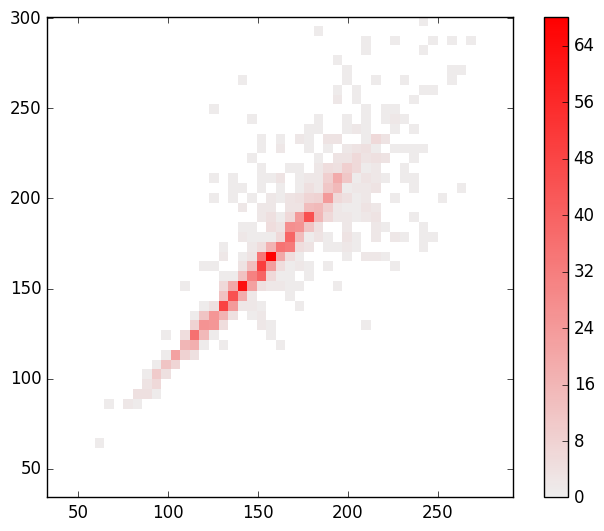
\includegraphics[scale=0.4]{img_size/lamellarity/heatmap_multilamellar.png} & 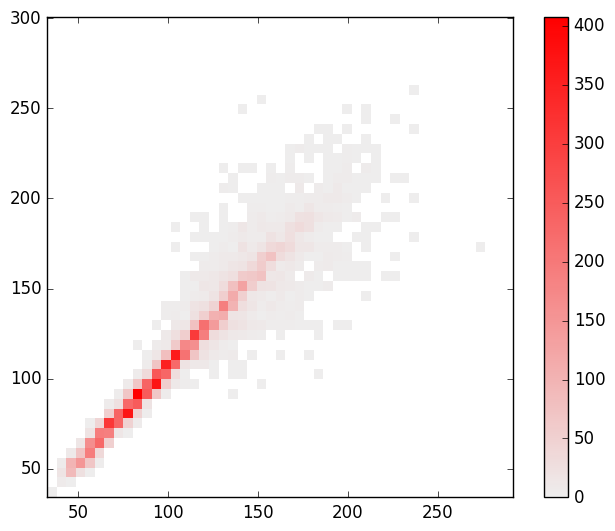
\includegraphics[scale=0.4]{img_size/lamellarity/heatmap_unilamellar.png} & 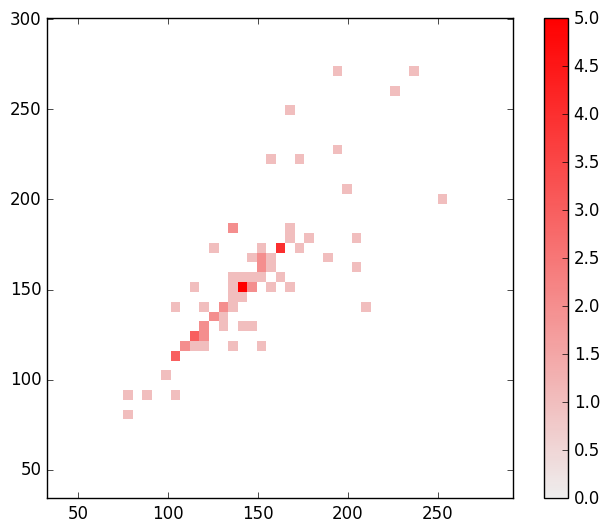
\includegraphics[scale=0.4]{img_size/lamellarity/heatmap_uncertain.png} \\
	Multilamellar & Unilamellar & Uncertain \\[6pt]
	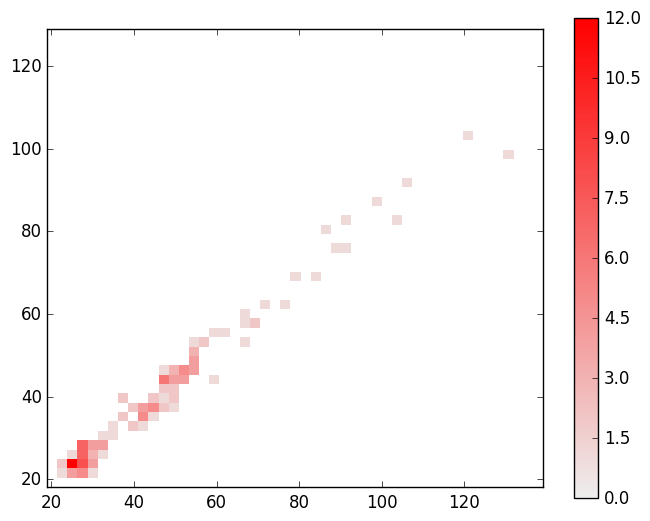
\includegraphics[scale=0.4]{img_size/encapsulation/heatmap_empty.png} & 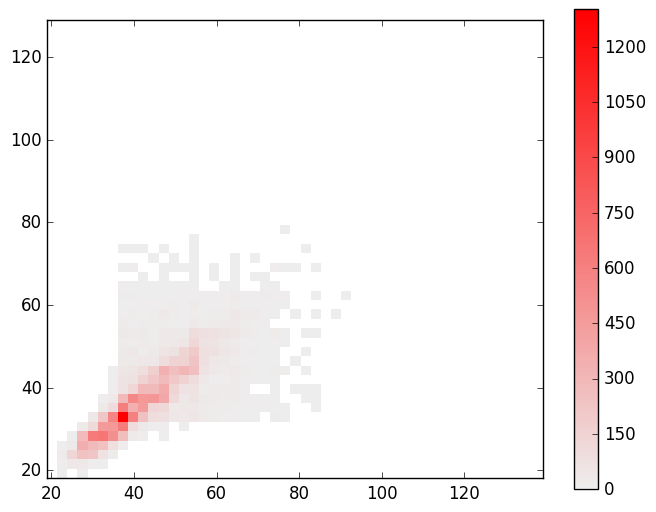
\includegraphics[scale=0.4]{img_size/encapsulation/heatmap_full.png} & 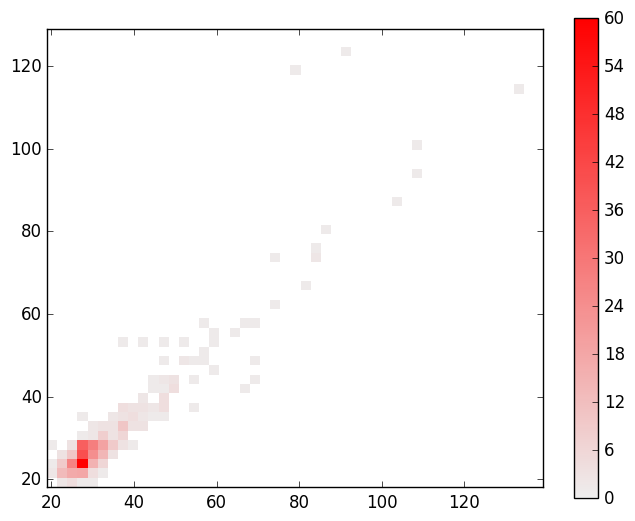
\includegraphics[scale=0.4]{img_size/encapsulation/heatmap_uncertain.png} \\
	Empty & Full & Uncertain \\[6pt]
\end{tabular}
\caption{Distribution of image sizes in each class. Upper row corresponds to lamellarity problem, lower corresponds to encapsulation problem.}
\label{fig:img_size_per_class}
\end{figure}
\end{landscape}


\section{Methodology}

\subsection{Support Vector Machines}
\label{sec:svm}
The support vector machine (SVM) is one of the most influential approaches to supervised learning~\cite{Boser:1992:TAO:130385.130401}. SVM is driven by a linear function $w^\top x + b$~\cite{dl_book}. In classification tasks SVM has the aim to determine decision boundaries that produce optimal class separation. SVM was initially designed for binary classification case but a number of modifications had been introduced for multiclass classification. On of them is "one-against-one" approach~\cite{Knerr1990}. According to this technique $n (n-1)\frac{1}{2}$, where $n$ is number of classes, classifiers are trained for each class. SVM does not provide probabilities, just a class identity~\cite{dl_book}. \texttt{LIBSVM}~\cite{CC01a} library is used for experiments in this project and it implements "one-against-one" technique.

Currently automatic classification is performed by means of SVM at Vironova. Performance of SVM method has shown up to $98\%$ accuracy on lamellarity problem and up to $87\%$ on encapsulation problem. The following features are used by Vironova:
\begin{itemize}
\item Area
\item Circularity
\item Image moments $\mu_{20}$, $\mu_{02}$, $\mu_{30}$, $\mu_{03}$
\item Edge density profile
\item Histogram
\item Internal segmentation variance
\end{itemize}

All named above features except internal segmentation variance are described in section~\ref{sec:dataset}. Internal segmentation variance is not available in provided data sets but its absence had insignificant impact on experiment results as shown later in this report.  

\subsection{Convolutional Neural Networks}
Convolutional networks~\cite{LeCun1986}, also known as convolutional neural networks or CNNs, are defined in~\cite{dl_book} as \blockquote{a specialized kind of neural network for processing data that has a known, grid-like topology. Convolutional networks are simply neural networks that use convolution in place of general matrix multiplication in at least one of their layers.}

Employing of CNNs for this project as the main tool for performing classification tasks is motivated in the following way. 

Since introduction in~\cite{LeCun1986} in the late 1980's, CNNs have demonstrated excellent performance in object detection and recognition tasks. One of the most influential applications of CNNs is ImageNet 2012 competition that was won using a CNN model~\cite{NIPS2012_4824} with error rate of $16.4\%$ which was a breakthrough at that time. There are also examples of successful application of CNNs in microscopy images domain. For example U-Net~\cite{Ronneberger2015} has solved biomedical image segmentation task provided very limited training data set. Area of CNNs application is extensive and they are being used by all leading IT companies such as Google, Facebook, Microsoft and others. Current interest for CNNs is driven mainly by three factors~\cite{Zeiler2014}: the availability of large annotated data sets; powerful GPU hardware and better model regularization strategies. 

CNNs are of great interest in image analysis domain because they allow unsupervised learning of image features. One does not need to be an image analysis specialist to build a powerful and robust image classification or object recognition system. Unlike many other methods of image analysis CNNs do not require handcrafted convolutional filters carefully designed by an image analysis specialist, even though these features can be incorporated in a CNN model. For instance, lamellarity and encapsulation problems have already been successfully solved by Vironova specialists using SVM and carefully selected image features such as area, circularity, image moments and other discussed in section~\ref{sec:svm}. This projects studies CNNs ability to achieve comparable result in fully unsupervised manner. 


\subsection{Deconvolutional Neural Networks}
Study and discuss deconvolutional networks~\cite{Zeiler2014} or other more basic visualization techniques and their use as potential aids for Vironova in deciding useful particle features to extract.

\subsection{Performance measures}

When evaluating a classification model one is almost always interested in how many predictions from all predictions made are correct. In other words we are interested in how accurate a particular model is. The accuracy of a classification system is the share of correct predictions in total number of examples. Accuracy  is one of the most frequently used performance measures in classification problems. However accuracy alone is usually not enough to describe predictive power of the model. Models with a given accuracy may have greater predictive power than models with higher accuracy. This is known as Accuracy Paradox~\cite{zhu2007knowledge}.

Let's illustrate Accuracy Paradox using encapsulation problem. Table~\ref{table:encapsulation_dataset} on page~\pageref{table:encapsulation_dataset} presents distribution of three classes in encapsulation data set. Consider a model that classifies all particles as full. Such model would achieve astonishing accuracy of $97\%$ just by making the same prediction for all particles. Let's compare it to another model, that makes a random guess, i.e. predicts each class with $\frac{1}{3}$ probability. Such random guess model would have accuracy of approximately $33\%$, almost three times less than the first model. However, while the first model totally ignores two minority classes, the second one has $33\%$ chance of detecting them, so it may be preferred comparing to the first one. 

Imbalanced data sets is a typical example when accuracy is misleading and fails as a performance measure. An unambiguous way to present the prediction results of a classification model is a confusion matrix~\cite{STEHMAN199777}. Confusion matrix is a table with number of rows and columns that are both equal to number of classes in the data set under consideration. Columns represent predicted classes and rows represent true classes. Each cell contains the number of predictions that corresponds to that particular category. 

A table of confusion is a special case of confusion matrix that is dealing with binary classification. Table of confusion is presented in table~\ref{table:table_of_confusion} and it is usually used to illustrate performance measures that are derived from confusion matrix.

\begin{center}
\captionof{table}{Table of confusion}
\label{table:table_of_confusion}
\begin{tabular}{|c|c|c|}
\hline 
 & Predicted True & Predicted False \\ 
\hline 
Actual True & \specialcell{True positive \\ TP} & \specialcell{False negative \\ FN} \\ 
\hline 
Actual False & \specialcell{False positive \\ FP} & \specialcell{True negative \\ TN} \\ 
\hline 
\end{tabular} 
\end{center}
 
Different performance measures are discussed and compared in~\cite{powers07evaluation}. The rest of this section presents performance measures that are used in this project for evaluation and comparing of different classification models. 

\textbf{True positive rate (TPR)}, also known as sensitivity or recall, measures share of positives that have been correctly identified:
\begin{equation*}
TPR = \frac{TP}{TP + FN}
\end{equation*}

\textbf{True negative rate (TNR)}, also known as specificity, measures share of negatives that have been correctly identified:
\begin{equation*}
TNR = \frac{TN}{TN + FP}
\end{equation*}

\textbf{Positive predicted value (PPV)}, also known as precision, measures share of correct positive predictions :
\begin{equation*}
PPV = \frac{TP}{TP + FP}
\end{equation*}

\textbf{Negative predicted value (NPV)}, measures share of correct negative predictions:
\begin{equation*}
NPV = \frac{TN}{TN + FN}
\end{equation*}

Presented above measures allow more detailed analysis of classifier performance and can clearly illustrate eventual bias of a classifier towards some class or classes. 

\subsection{Class Imbalance Problem}
\label{sec:class_imbalance}
Encyclopedia of Machine Learning~\cite{Ling2010} defines Class Imbalance problem as follows:
\blockquote{Data are said to suffer the \textit{Class Imbalance Problem} when the class distributions are highly imbalanced. In this context, many classification learning algorithms have low predictive accuracy for the infrequent class.}

It is a serious problem because most machine learning algorithms will tend to classify all examples as majority class treating examples of minority class as noise. Lamellarity and encapsulation data sets presented in sections~\ref{sec:lamellarity} and~\ref{sec:encapsulation} respectively are highly unbalanced. In lamellarity data set majority class accounts for $87\%$ of all samples and in encapsulation dataset majority class constitutes $97\%$ of all samples. Preliminary experiments showed that classifiers trained on raw unbalanced data sets are highly biased towards majority classes and do not generalize. Imbalance problem is not uncommon. In fact, data sets are highly imbalanced in many domains, for example fraud detection, medical diagnosis, anomaly detection, telecommunications, etc. 

Various solutions have been proposed to deal with this problem and they can be summarized into three groups~\cite{Lopez2013113}:

\begin{itemize}

\item \textit{Data sampling} implies any means to produce more or less balanced data set. For example it can be oversampling, undersampling, SMOTE~\cite{smote_chawla} or generating artificial examples~\cite{ishaq_synthetic}. Data sampling method perform usually best combined with data augmentation techniques.

\item \textit{Algorithm modification} this procedure is oriented towards the adaptation of base learning methods to be more attuned to class imbalance issues ~\cite{Zadrozny:2001:LMD:502512.502540}.

\item \textit{Cost sensitive learning} introduces higher penalties for misclassification of minority classes making learning algorithm more sensitive to underrepresented classes. 

\end{itemize}

Listed above methods prevent classifiers from ignoring underrepresented classes during training phase. However this is very likely to lead to another problem --- overfitting. Overfitting and how to combat it is discussed in section~\ref{sec:regularization}. The rest of this section discusses methods that have been used to mitigate Class Imbalance Problem in lamellarity and encapsulation data sets. 


\subsubsection{Oversampling}
Oversampling means repeating instances of underrepresented classes. Minority classes in lamellarity data set are multilamellar and uncertain, and in encapsulation data set --- empty and uncertain. Examples of these classes are repeated to match number of training samples of majority class so training sets become balanced. Oversampling itself does not mitigate imbalance problem much, it works best combined with data augmentation which is discussed in section~\ref{sec:data_augmentation}.

\subsubsection{Undersampling}
Undersampling, as opposed to oversampling, means excluding some examples of majority class in order to make training set balanced. In practice undersampling is repeated at the beginning of each learning epoch when randomly selected examples are excluded. In such way learning algorithm can still use all samples for training, it just does not see all of them during all epochs. Proportion of excluded examples can vary and depends on the contexts. In experiments presented in this project undersampling implies dropping $20\%$ of majority class examples. 

\subsubsection{SMOTE}
Synthetic Minority Over-sampling Technique (SMOTE) is an over-sampling approach in which the minority class is over-sampled by creating “synthetic” examples rather than by over-sampling with replacement~\cite{smote_chawla}. 
Synthetic examples are generated by combining each minority class example with its randomly selected $k$ nearest neighbors, where $k$ is a parameter that depends on amount of required over-sampling.

\subsubsection{Artificial data}
Machine learning algorithms perform best provided large training data sets. In many domains, including medicine and biology, expert annotation is required for preparing training and test data sets. This results in high cost and effort, so size of data sets if often limited. In such case artificial artificial data is an attractive alternative to real expert-annotated data. Training of convolutional neural network models for fluorescent spot detection on artificial data is discussed and evaluated in~\cite{ishaq_synthetic}. 

\begin{figure}[H]
\centering
\begin{tabular}{ccc}
	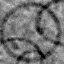
\includegraphics[scale=1.5]{synthetic/uni.png} & 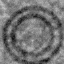
\includegraphics[scale=1.5]{synthetic/multi.png} & 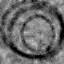
\includegraphics[scale=1.5]{synthetic/uncertain.png} \\
	Unilamellar & Multiilamellar & Uncertain \\[6pt]
\end{tabular}
\caption{Artificial examples, lamellarity problem}
\label{fig:synthetic_images}
\end{figure}

In this project artificial data has been generated for lamellarity problem. Artificial EM images of liposomes are generated by drawing circles with carefully selected randomized distortions. Background and distortions are generated using Perlin noise~\cite{Perlin:1985:IS:325165.325247}. Figure~\ref{fig:synthetic_images} presents examples of artificially generated EM images.

Note that despite visual similarity artificial images are not based on statistical measures from real data set. Histograms and image patterns are not drawn from real distributions. With limited time and effort, this experiment should be rather seen as a proof of concept.


\section{Regularization}
\label{sec:regularization}

Let us assume that an imbalanced data set has been balanced by any combination of methods described in section~\ref{sec:class_imbalance}. This would significantly reduce training error which means that the model is able to describe data generation process of the training set. 

However as the result of seeing multiple copies of minority classes learning algorithm will almost likely describe random error or noise as well. Such model would not be able to make reliable predictions on general untrained data, i. e. its generalization error would still be unacceptably high. As defined in~\cite{dl_book} \blockquote{\textit{Generalization} is any modification we make to a learning algorithm that is intended to reduce its generalization error but not its training error}.

The reset of this section presents regularization techniques that have been used to reduce generalization error of models trained on lamellarity and encapsulation data sets.

\subsection{Weight decay}
Weight decay is a method of adding penalty on hidden layer weights magnitude to the loss function. In this way we express preference of smaller weights and prevent weight of some hidden nodes or convolutional filters from becoming to large. Large weights can result in undesired numerical errors such as overflow or truncation error. Usually $L^2$ norm of penalized layers multiplied by some constant $\alpha$ (typically close to zero) is added to the loss function. However other norms such as but not limited to $L^1$ can be used. 
On the other hand weight decay can lead to other problems as described in~\cite{dl_book}. Penalties on weights can cause non-convex optimization procedures to get stuck in local minima corresponding to small values of weights. 

Applied to neural networks it means that weight decay can lead to \blockquote{dead units}. These units do not contribute much to the learning process because their input and output weights are all very small. This configuration can be locally optimal even if loss value can be significantly reduced by making the wights larger. This fenomena was observed during experiments presented in this project. Applying weight decay to convolutional layers resulted in numerous dead filters which worsened classifiers performance on both training and test sets.

\subsection{Noise injection}
Noise robustness can be achieved by adding some noise to the model. Noise can be added at several places. 

Firstly, noise can be added to the input, in our case to EM images. However EM images are generally quite noisy while some examples are very noisy. 

Secondly, noise can be added to weights. This technique is primarily used in recurrent neural networks~\cite{jim1996}. 

Thirdly, most data sets have some mistakes in the annotated labels. As shown in section~\ref{sec:loss_function}, it can be very costly to maximize $\log p(y|x)$ when label $y$ is wrong. Label smoothing technique is proposed in~\cite{dl_book}. Label smoothing regularizes a model based on a softmax with $k$ output values by replacing the hard 0 and 1 classification targets with targets of $\frac{\epsilon}{k}$ and $1 - \frac{k-1}{k}\epsilon$, respectively, where $\epsilon$ is an arbitrary value between 0 and 1, usually very close to 0. Label smoothing operation is summarized in equation~\ref{eq:soft_targets}.

\begin{equation}
\label{eq:soft_targets}
x \leftarrow x \left( 1 - \epsilon \right) + \left(1 - x\right) \frac{\epsilon}{k - 1}
\end{equation}

Label smoothing is used in all experiments presented in this project.

\subsection{Dropout}
Dropout~\cite{JMLR:v15:srivastava14a} suggests to randomly drop non--output units (nodes) along with their connections from the network. This prevents units from co--adapting too much. Dropout is implemented as a parameter between $0$ and $1$ that describes probability of dropping each unit. It can be constant during all training epochs or some decay scheme may be used. Dropout may be more aggressive in the beginning of training and smaller later when the model becomes trained, it is the same idea as with learning rate decay. Dropout is used in all experiments presented in this project.


\subsection{Early stopping}
Early stopping is probably the most commonly used regularization strategy in deep learning~\cite{dl_book}. It is a simple yet powerful technique of determining optimal number of training epochs. Idea is to split training data into train set used to train the model and validation set, which is not used in training process. Errors of both sets are monitored at each epoch. Training should be stopped when validation set performance has not improved for some selected number of epochs. This prevents overfitting and improves generalization. Validation set error is more suitable than training set error because training error decreases steadily over time as model starts to overfit while validation error begins to rise again. 
In this project early stopping is used to determine number of training epochs, that is later fixed during k-fold cross validation.

\subsection{Data augmentation}
\label{sec:data_augmentation}
As was already mentioned in section~\ref{sec:class_imbalance} training data is often limited and additional data is hard to obtain. One way to get around this problem is to introduce additional diversity in training set by augmenting existing data. Data augmentation has proven to be especially effective for classification tasks~\cite{dl_book} which is exactly the case in this project. 
A good classifier is invariant to a wide variety of transformations and can see true class from \blockquote{different points of view}. New $(x, y)$ pairs, where $x$ is a class example and $y$ is corresponding label, can be easily generated by applying different transformations to $x$. Choice of transformations is highly application dependent. For example, optical recognition models must recognize difference between `b' and `d' and between `6' and `9', so horizontal and vertical flips are not suitable for this task. 
 

In this project data is augmented in the following way:
\begin{itemize}
\item Rotation in range $(-180, 180)$ degrees with spline interpolation
\item Shear transformation
\item Vertical shift in range $(-10, 10)$ percent of total height
\item Horizontal shift in range $(-10, 10)$ percent of total width
\item Zoom
\item Horizontal flip
\item Vertical flip
\end{itemize}

All transformations are applied randomly. Horizontal and vertical flips are performed with $50\%$ probability, rotation, shear, shift and zoom values are uniform random integer values in specified ranges. Data augmentation is performed in all experiments unless the opposite is stated explicitly.

\section{Loss function}
\label{sec:loss_function}

\begin{warning}
This section is taken from project report for Machine Learning course. How to cite it?
\end{warning}

The multi-class logarithmic loss function is a loss function that represents the price paid for inaccuracy of predictions in classification problems~\cite{rosasco}. The formula is:
\begin{equation}
loss = -\frac{1}{N} \sum_{i=1}^{N} \sum_{j=1}^{M} y_{i,j} log(p_{i,j})
\end{equation}

Where 
\begin{itemize}
\item N -- number of observations
\item M -- number of classes, it is five in our case
\item \textit{log} -- natural logarithm
\item $y_{i,j}$ -- is 1 if observation $i$ is in class $j$ and 0 otherwise
\item $p_{i,j}$ --  is the predicted probability that observation $i$ is in class $j$
\end{itemize}

In order to calculate multi-class logarithmic loss the classifier must assign a probability to each class rather than simply yielding the most likely class. This fact constitutes the main difference between accuracy and logarithmic loss. In order to consider a prediction as accurate, it is sufficient that classifier marks the correct class as the most likely one, no matter how confident the prediction is.

Figure~\ref{fig:logloss} shows log loss from a single class where predicted probability ranges from 0 (the completely wrong prediction) to 1 (the correct prediction). As predicted probability moves closer to 1, log loss decreases gently to 0. On the contrary, log loss increases rapidly as predicted probability moves towards zero. It is clear from Figure~\ref{fig:logloss} that the multi-class logarithmic loss heavily penalizes classifiers that are confident about an incorrect classification.

\begin{figure}[H]
\centering
\begin{tikzpicture}
\begin{axis}[
	axis lines = left,
	xlabel = Predicted probability,
	ylabel = Loss,
]
\addplot [
	domain=0.0001:1,
	samples=100,
	color=red,
]
{-ln(x)};
\addlegendentry{$f(x) = -log(x)$}
\end{axis}
\end{tikzpicture}
\caption{\label{fig:logloss} Log loss of a single class where predicted probability ranges from 0 to 1. }
\end{figure}

Consider an example of a binary classifier and let us take a look at the effect of various predictions for class membership probability. 
\begin{itemize}
\item Classification that assigns equal probabilities to both classes results in loss $-log(0.5)=0.6932$.  

\item Classification confident in the correct class results in loss $-log(0.9)=0.1054$.

\item Classification confident in the wrong class results in loss $-log(0.1)=2.3026$. 
\end{itemize}

In other words, the log loss function encourages moderate predictions. It is better to make all classifications neutral rather than make 50\% correct classifications and 50\% completely wrong predictions.

\section{Implementation of CNN}

\subsection{Convolutional layer network}

Model configuration:
\begin{itemize}
\item Convolutional layer, 32 kernels, relu activation
\item Convolutional layer, 32 kernels, relu activation
\item Max pooling
\item Dropout
\item Convolutional layer, 64 kernels, relu activation
\item Convolutional layer, 64 kernels, relu activation
\item Max pooling
\item Dropout
\item Dense layer, 512 nodes, relu ctivation
\item Dropout
\item Dense layer, 3 nodes, softmax activation

\end{itemize}

\subsubsection{K-fold cross validation}

\begin{landscape}
\begin{table}
\caption{5-fold cross validation, CNN, Lamellarity problem.} \label{t:kfold-cnn-lamellarity}

\smallskip
\begin{tabular*}{\linewidth}{@{} l @{\extracolsep{\fill}} *{12}{S[table-format=2.1]}
                                 *{4}{S[table-format=2.1]} @{}}
\toprule
 & \multicolumn{4}{c}{Unilamellar} & \multicolumn{4}{c}{Multilamellar} 
         & \multicolumn{4}{c}{Uncertain}  \\
\cmidrule(lr){2-5} \cmidrule(lr){6-9} \cmidrule(lr){10-13}  
Fold & \mcc{TPR} & \mcc{SPC} & \mcc{PPV} & \mcc{NPV} & \mcc{TPR} & \mcc{SPC} & \mcc{PPV} & \mcc{NPV} & \mcc{TPR} & \mcc{SPC} & \mcc{PPV} & \mcc{NPV}  \\
\midrule
1 & 0.8634 & 0.9972 & 0.9995 & 0.5158 & 0.9797 & 0.9542 & 0.7472 & 0.9971 & 0.5294 & 0.9155 & 0.0364 & 0.9969\\
2 & 0.9107 & 0.9917 & 0.9987 & 0.6183 & 0.9913 & 0.9683 & 0.8119 & 0.9988 & 0.4706 & 0.9464 & 0.0503 & 0.9966\\
3 & 0.9798 & 0.9945 & 0.9992 & 0.8778 & 1.0000 & 0.9912 & 0.9399 & 1.0000 & 0.4706 & 0.9876 & 0.1860 & 0.9968\\
4 & 0.9915 & 0.9945 & 0.9992 & 0.9447 & 0.9884 & 0.9972 & 0.9798 & 0.9984 & 0.8235 & 0.9933 & 0.4242 & 0.9989\\
5 & 0.8956 & 0.9972 & 0.9995 & 0.5798 & 0.9707 & 0.9803 & 0.8711 & 0.9959 & 0.7500 & 0.9211 & 0.0513 & 0.9985\\
\midrule
Avg & 0.9282 & 0.9950 & 0.9992 & 0.7073 & 0.9860 & 0.9782 & 0.8700 & 0.9980 & 0.6088 & 0.9528 & 0.1497 & 0.9975\\ 
\bottomrule
\end{tabular*}
\end{table}

\begin{table}
\caption{5-fold cross validation, CNN, Encapsulation problem.} \label{t:kfold-cnn-encapsulation}

\smallskip
\begin{tabular*}{\linewidth}{@{} l @{\extracolsep{\fill}} *{12}{S[table-format=2.1]}
                                 *{4}{S[table-format=2.1]} @{}}
\toprule
 & \multicolumn{4}{c}{Empty} & \multicolumn{4}{c}{Full} 
         & \multicolumn{4}{c}{Uncertain}  \\
\cmidrule(lr){2-5} \cmidrule(lr){6-9} \cmidrule(lr){10-13}  
Fold & \mcc{TPR} & \mcc{SPC} & \mcc{PPV} & \mcc{NPV} & \mcc{TPR} & \mcc{SPC} & \mcc{PPV} & \mcc{NPV} & \mcc{TPR} & \mcc{SPC} & \mcc{PPV} & \mcc{NPV}  \\
\midrule
1 & 0.3030 & 0.9917 & 0.1961 & 0.9953 & 0.8194 & 0.8358 & 0.9945 & 0.1134 & 0.7624 & 0.8239 & 0.0822 & 0.9941\\
2 & 0.3030 & 0.9861 & 0.1266 & 0.9953 & 0.9019 & 0.7761 & 0.9932 & 0.1793 & 0.5149 & 0.9081 & 0.1038 & 0.9891\\
3 & 0.4545 & 0.9849 & 0.1667 & 0.9963 & 0.8992 & 0.8955 & 0.9968 & 0.1970 & 0.7030 & 0.9083 & 0.1368 & 0.9933\\
4 & 0.6061 & 0.9895 & 0.2778 & 0.9974 & 0.9427 & 0.7836 & 0.9937 & 0.2742 & 0.6139 & 0.9490 & 0.1994 & 0.9917\\
5 & 0.8276 & 0.9861 & 0.2581 & 0.9990 & 0.9258 & 0.9291 & 0.9980 & 0.2469 & 0.5510 & 0.9322 & 0.1403 & 0.9904\\
\midrule
Avg & 0.4989 & 0.9876 & 0.2050 & 0.9967 & 0.8978 & 0.8440 & 0.9952 & 0.2021 & 0.6290 & 0.9043 & 0.1325 & 0.9917\\ 
\bottomrule
\end{tabular*}
\end{table}

\end{landscape}

\subsubsection{Visualization, Lamellarity problem}

\begin{figure}[H]
\begin{tabular}{cc}
	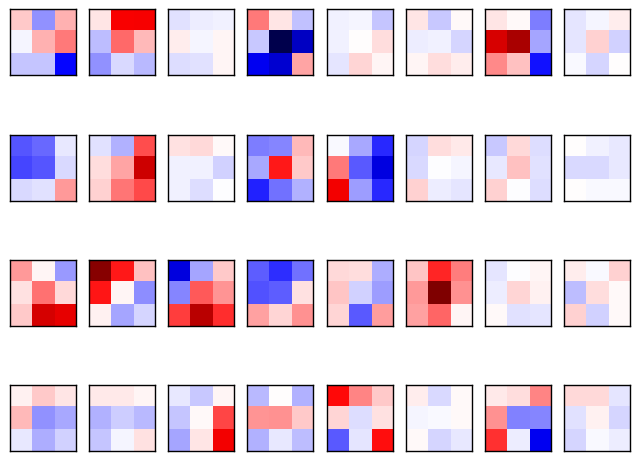
\includegraphics[scale=0.4]{models/cnn_deep/weights/convolution2d_1-0.png} & 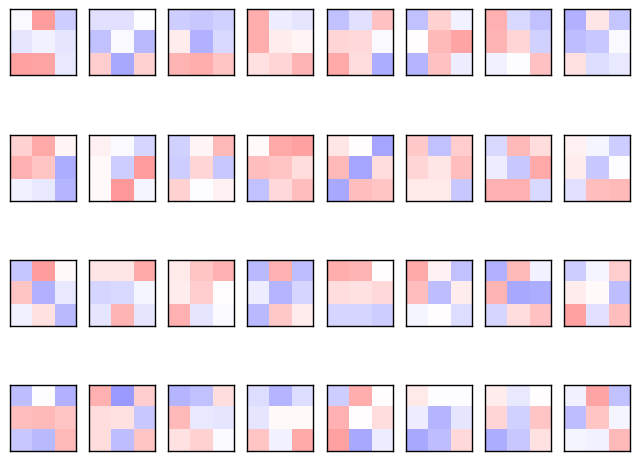
\includegraphics[scale=0.4]{models/cnn_deep/weights/convolution2d_2-23.png} \\
	\rom{1} & \rom{2}, channel 24 \\[6pt]
	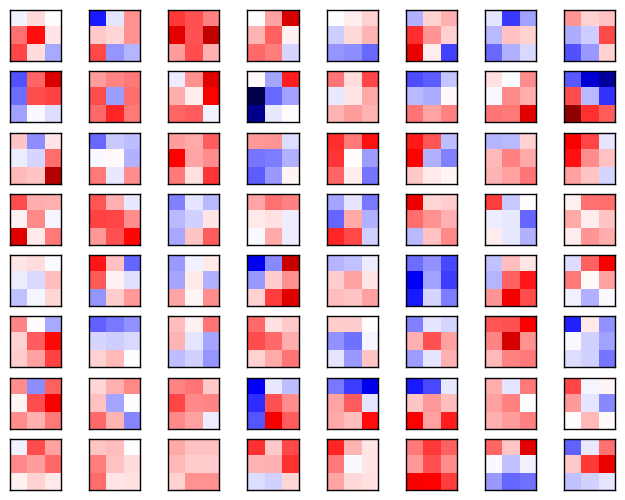
\includegraphics[scale=0.4]{models/cnn_deep/weights/convolution2d_3-3.png} & 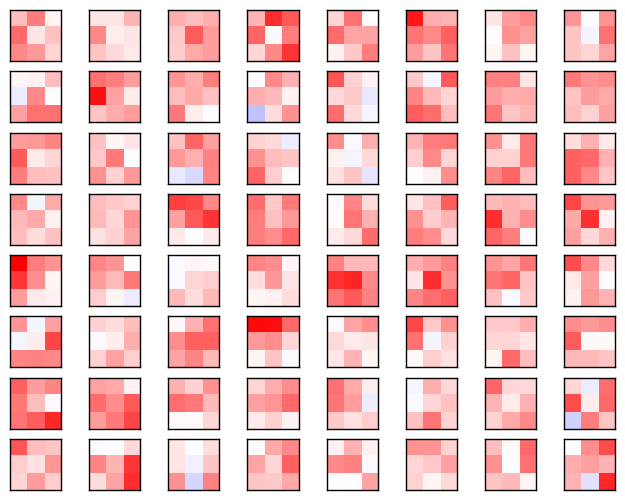
\includegraphics[scale=0.4]{models/cnn_deep/weights/convolution2d_4-58.png} \\
	\rom{3}, channel 4 & \rom{4}, channel 59 \\[6pt]
\end{tabular}
\caption{Visualization of convolution kernels}
\end{figure}

\begin{figure}[H]
\begin{tabular}{cc}
	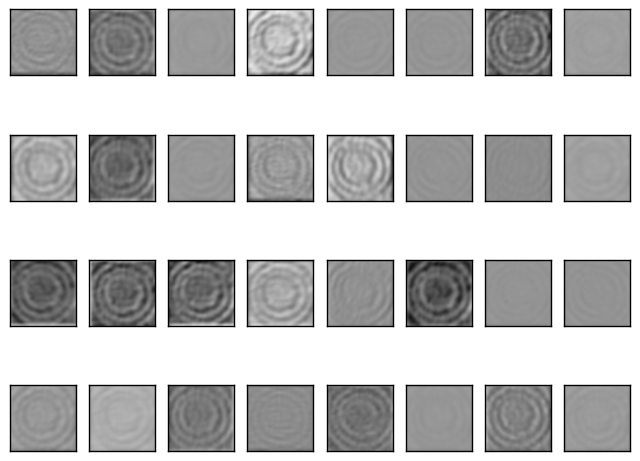
\includegraphics[scale=0.4]{models/cnn_deep/output/convolution2d_1.png} & 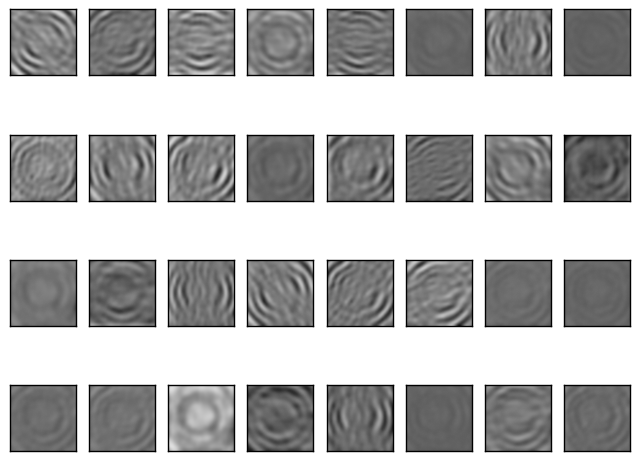
\includegraphics[scale=0.4]{models/cnn_deep/output/convolution2d_2.png} \\
	\rom{1} & \rom{2} \\[6pt]
		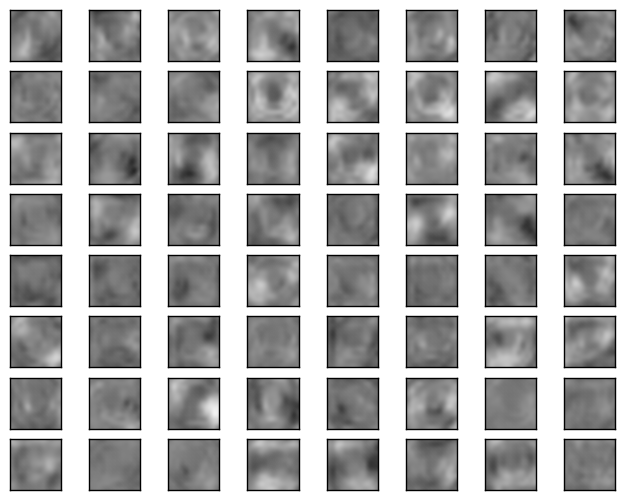
\includegraphics[scale=0.4]{models/cnn_deep/output/convolution2d_3.png} & 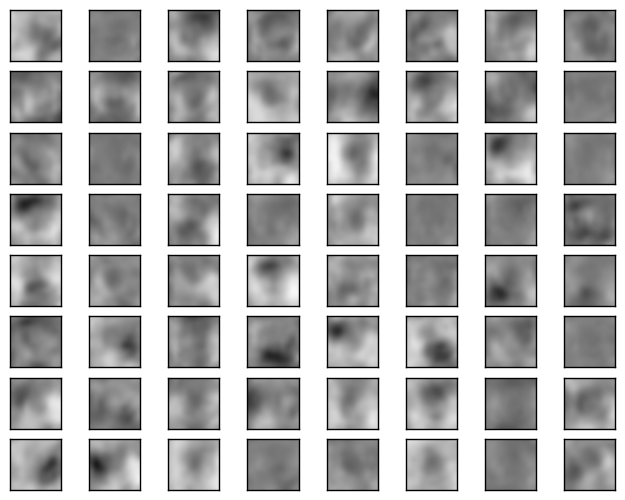
\includegraphics[scale=0.4]{models/cnn_deep/output/convolution2d_4.png} \\
	\rom{3} & \rom{4} \\[6pt]

\end{tabular}
\caption{Visualization of convolutional layers outputs}
\end{figure}



\subsection{Review of deep learning software libraries}

Deep learning software tool have been benchmarked in~\cite{benchmarking_dl_tools}

\begin{landscape}
\begin{center}
\captionof{table}{Comparison of characteristics of deep learning frameworks}
\begin{tabular}{lccccccccl}
\hline 
 & \multicolumn{2}{c}{\cellcolor{linux}Linux} & \multicolumn{2}{c}{\cellcolor{windows}Windows} & \multicolumn{2}{c}{\cellcolor{macos}Mac OS} & \multicolumn{2}{c}{Language bindings} &  \\ 
 & \cellcolor{linux}CPU & \cellcolor{linux}GPU & \cellcolor{windows}CPU & \cellcolor{windows}GPU & \cellcolor{macos}CPU & \cellcolor{macos}GPU & Python & C++ & License\\ 
\hline 
Caffe & \ymark & \ymark & \ymark & \ymark & \ymark & \ymark & \ymark & \nmark & BSD 2\\ 
cntk & \ymark & \ymark & \ymark & \ymark & \nmark & \nmark & \ymark & \ymark & Custom\footnote{Allows commercial use \textcolor{red}{reference}} \\ 
Keras & \ymark & \ymark & \ymark & \ymark & \ymark & \ymark & \ymark & \nmark & MIT \\ 
Lasagne & \ymark & \ymark & \ymark & \ymark & \ymark & \ymark & \ymark & \nmark & MIT \\ 
mxnet & \ymark & \ymark & \ymark & \ymark & \ymark & \ymark & \ymark & \ymark & Apache 2.0 \\ 
nolearn & \ymark & \ymark & \ymark & \ymark & \ymark & \ymark & \ymark & \nmark & MIT \\ 
Tensorflow & \ymark & \ymark & \nmark & \nmark & \ymark & \nmark & \ymark & \ymark & Apache 2.0 \\ 
Theano & \ymark & \ymark & \ymark & \ymark & \ymark & \ymark & \ymark & \nmark & BSD 3\\ 
\end{tabular} 
\end{center}

\begin{center}
\captionof{table}{Comparison of popularity of deep learning frameworks}
\begin{tabular}{lrrrrr}
\hline 
 & \multicolumn{4}{c}{Github} & Stackoverflow \\ 
 & Contributors & Stars & Forks & Subscribers & Questions \\ 
\hline 
Caffe & 208 & 12349 & 7513 & 1559 & 1038 \\ 
cntk & 77 & 6181 & 1343 & 688 & 12 \\ 
Keras & 257 & 8044 & 2470 & 639 & 444 \\ 
Lasagne & 51 & 2452 & 673 & 202 & 153 \\ 
mxnet & 174 & 4969 & 1887 & 559 & 22 \\ 
nolearn & 9 & 718 & 203 & 52 & 44 \\ 
Tensorflow & 380 & 31445 & 13414 & 2983 & 3275 \\ 
Theano & 251 & 4475 & 1609 & 424 & 1436 \\ 
\end{tabular} 
\end{center}



\end{landscape}

\section{Results}

\subsection{Confusion matrix}

\begin{warning}
Average confusion matrix from k-fold cross validation. Does it make sense? 
\end{warning}

% CNN
\begin{center}
\captionof{table}{Lamellarity problem, fold 5, CNN}
\begin{tabular}{lrrr}
\hline
 & Unilamellar & Uncertain & Multilamellar \\ 
\hline 
Unilamellar & 0.90 & 0.01 & 0.09 \\ 
Multilamellar & 0.00 & 0.97 & 0.03 \\ 
Uncertain & 0.00 & 0.25 & 0.75 \\ 
\end{tabular} 
\end{center}

% SVM
\begin{center}
\captionof{table}{Lamellarity problem, fold 5, SVM}
\begin{tabular}{lrrr}
\hline
 & Unilamellar & Uncertain & Multilamellar \\ 
\hline 
Unilamellar & 0.87 & 0.03 & 0.10 \\ 
Multilamellar & 0.02 & 0.95 & 0.03 \\ 
Uncertain & 0.03 & 0.00 & 0.97 \\ 
\end{tabular} 
\end{center}

% CNN
\begin{center}
\captionof{table}{Encapsulation problem, fold 5, CNN}
\begin{tabular}{lrrr}
\hline
 & Empty & Full & Uncertain \\ 
\hline 
Empty & 0.83 & 0.07 & 0.10 \\ 
Packed & 0.01 & 0.93 & 0.06 \\ 
Uncertain & 0.38 & 0.07 & 0.55 \\ 
\end{tabular} 
\end{center}

% SVM
\begin{center}
\captionof{table}{Encapsulation problem, fold 5, SVM}
\begin{tabular}{lrrr}
\hline
 & Empty & Full & Uncertain \\ 
\hline 
Empty & 0.93 & 0.01 & 0.06 \\ 
Packed & 0.04 & 0.87 & 0.09 \\ 
Uncertain & 0.25 & 0.12 & 0.63 \\ 
\end{tabular} 
\end{center}

\subsection{K-fold cross validation}

\subsection{SVM}

\begin{landscape}

\begin{table}
\caption{5-fold cross validation, SVM, Lamellarity problem.} \label{t:kfold-svm-lamellarity}

\smallskip
\begin{tabular*}{\linewidth}{@{} l @{\extracolsep{\fill}} *{12}{S[table-format=2.1]}
                                 *{4}{S[table-format=2.1]} @{}}
\toprule
 & \multicolumn{4}{c}{Unilamellar} & \multicolumn{4}{c}{Multilamellar} 
         & \multicolumn{4}{c}{Uncertain}  \\
\cmidrule(lr){2-5} \cmidrule(lr){6-9} \cmidrule(lr){10-13}  
Fold & \mcc{TPR} & \mcc{SPC} & \mcc{PPV} & \mcc{NPV} & \mcc{TPR} & \mcc{SPC} & \mcc{PPV} & \mcc{NPV} & \mcc{TPR} & \mcc{SPC} & \mcc{PPV} & \mcc{NPV}  \\
\midrule
1 & 0.8659 & 0.9812 & 0.9969 & 0.5157 & 0.9527 & 0.9736 & 0.8326 & 0.9933 & 0.9851 & 0.9021 & 0.0565 & 0.9999 \\
2 & 0.8578 & 0.9826 & 0.9971 & 0.5014 & 0.9432 & 0.9719 & 0.8222 & 0.9920 & 0.9701 & 0.8951 & 0.0521 & 0.9998 \\
3 & 0.8404 & 0.9806 & 0.9966 & 0.4721 & 0.9432 & 0.9671 & 0.7979 & 0.9920 & 0.9701 & 0.8844 & 0.0475 & 0.9998  \\
4 & 0.8742 & 0.9757 & 0.9960 & 0.5302 & 0.9315 & 0.9721 & 0.8215 & 0.9904 & 0.9851 & 0.9088 & 0.0604 & 0.9999\\
5 & 0.8651 & 0.9806 & 0.9967 & 0.5147 & 0.9477 & 0.9695 & 0.8109 & 0.9926 & 0.9706 & 0.9045 & 0.0577 & 0.9998\\
\midrule
Avg & 0.8607 & 0.9801 & 0.9967 & 0.5068 & 0.9436 & 0.9708 & 0.8170 & 0.9921 & 0.9762 & 0.8990 & 0.0548 & 0.9998\\ 
\bottomrule
\end{tabular*}
\end{table}

\begin{table}
\caption{5-fold cross validation, SVM, Encapsulation problem.} \label{t:kfold-svm-encapsulation}

\smallskip
\begin{tabular*}{\linewidth}{@{} l @{\extracolsep{\fill}} *{12}{S[table-format=2.1]}
                                 *{4}{S[table-format=2.1]} @{}}
\toprule
 & \multicolumn{4}{c}{Empty} & \multicolumn{4}{c}{Full} 
         & \multicolumn{4}{c}{Uncertain}  \\
\cmidrule(lr){2-5} \cmidrule(lr){6-9} \cmidrule(lr){10-13}  
Fold & \mcc{TPR} & \mcc{SPC} & \mcc{PPV} & \mcc{NPV} & \mcc{TPR} & \mcc{SPC} & \mcc{PPV} & \mcc{NPV} & \mcc{TPR} & \mcc{SPC} & \mcc{PPV} & \mcc{NPV}  \\
\midrule
1 & 0.8750 & 0.9594 & 0.1223 & 0.9992 & 0.8703 & 0.9357 & 0.9980 & 0.1644 & 0.7082 & 0.9073 & 0.1356 & 0.9934\\
2 & 0.8984 & 0.9477 & 0.1000 & 0.9993 & 0.8625 & 0.9376 & 0.9980 & 0.1567 & 0.7681 & 0.9126 & 0.1529 & 0.9948\\
3 & 0.8828 & 0.9576 & 0.1186 & 0.9992 & 0.8582 & 0.9149 & 0.9973 & 0.1496 & 0.7207 & 0.8979 & 0.1266 & 0.9937\\
4 & 0.8516 & 0.9487 & 0.0969 & 0.9990 & 0.8676 & 0.9244 & 0.9976 & 0.1599 & 0.7980 & 0.9174 & 0.1655 & 0.9955\\
5 & 0.9318 & 0.9570 & 0.1263 & 0.9995 & 0.8666 & 0.9067 & 0.9970 & 0.1580 & 0.6337 & 0.9056 & 0.1218 & 0.9917\\
\midrule
Avg & 0.8879 & 0.9541 & 0.1128 & 0.9992 & 0.8650 & 0.9239 & 0.9976 & 0.1577 & 0.7257 & 0.9082 & 0.1405 & 0.9938\\ 
\bottomrule
\end{tabular*}
\end{table}

\end{landscape}

\subsection{ROC}
Include ROC curves of different models.

\section{Benchmarking}
\begin{warning}
Please comment selection of performance measures for benchmarking! 
\end{warning}

\begin{landscape}

\begin{figure}
\centering

% Empty
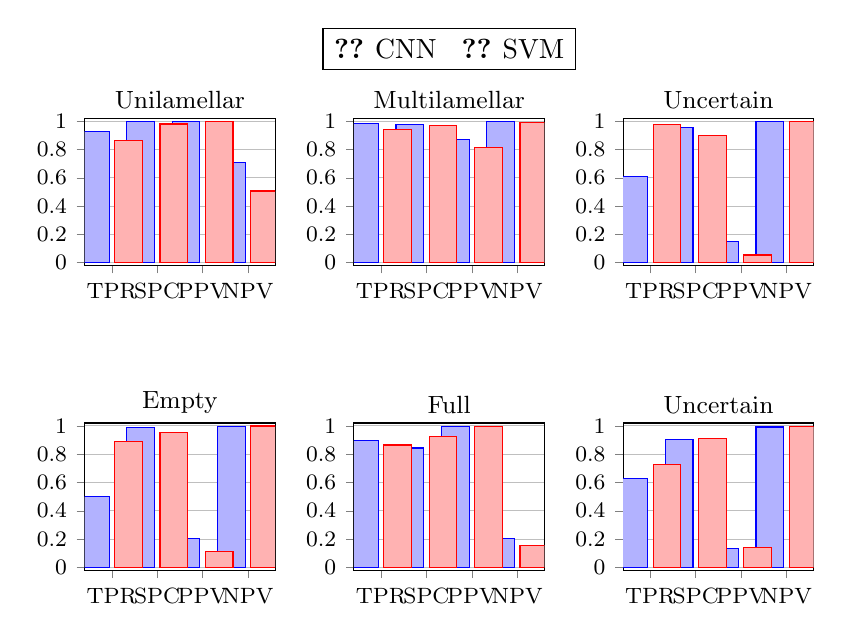
\begin{tikzpicture}
\begin{groupplot}[
	group style={
		group name=group_encapsulation,
		group size=3 by 2,
		ylabels at=edge left,
		vertical sep=2cm,
	},
	footnotesize,
	width=\linewidth * 0.33,
	%height=5cm,
	tickpos=left,
	ytick align=outside,
	xtick align=outside,
	enlarge x limits = 0.2,
	enlarge y limits = 0.02,
	xtick=data,
	enlarge x limits = 0.2,
	enlarge y limits = 0.02,
	ymin=0,
	ymax=1,
	legend style={at={(0.5,-0.1)},
	anchor=north,legend columns=-1},
	ybar,
	symbolic x coords={TPR, SPC, PPV, NPV},
	grid=major,
	xmajorgrids=false,
]
%
% Lamlellarity
%
\nextgroupplot[title={Unilamellar}]
% cnn
\addplot coordinates{(TPR, 0.9282) (SPC, 0.9950) (PPV, 0.9992) (NPV, 0.7073)};\label{legend:cnn}
% svm
\addplot coordinates{(TPR, 0.8607) (SPC, 0.9801) (PPV, 0.9967) (NPV, 0.5068)};\label{legend:svm}

\nextgroupplot[title={Multilamellar}]
% cnn
\addplot coordinates{(TPR, 0.9860) (SPC, 0.9782) (PPV, 0.8700) (NPV, 0.9980)};
% svm
\addplot coordinates{(TPR, 0.9436) (SPC, 0.9708) (PPV, 0.8170) (NPV, 0.9921)};

\nextgroupplot[title={Uncertain}]
% cnn
\addplot coordinates{(TPR, 0.6088) (SPC, 0.9528) (PPV, 0.1497) (NPV, 0.9975)};
% svm
\addplot coordinates{(TPR, 0.9762) (SPC, 0.8990) (PPV, 0.0548) (NPV, 0.9998)};

%
% Encapsulation
%
\nextgroupplot[title={Empty}]
% cnn
\addplot coordinates{(TPR, 0.4989) (SPC, 0.9876) (PPV, 0.2050) (NPV, 0.9967)};
% svm
\addplot coordinates{(TPR, 0.8879) (SPC, 0.9541) (PPV, 0.1128) (NPV, 0.9992)};

\nextgroupplot[title={Full}]
% cnn
\addplot coordinates{(TPR, 0.8978) (SPC, 0.8440) (PPV, 0.9952) (NPV, 0.2021)};
% svm
\addplot coordinates{(TPR, 0.8650) (SPC, 0.9239) (PPV, 0.9976) (NPV, 0.1577)};

\nextgroupplot[title={Uncertain}]
% cnn
\addplot coordinates{(TPR, 0.6290) (SPC, 0.9043) (PPV, 0.1325) (NPV, 0.9917)};
% svm
\addplot coordinates{(TPR, 0.7257) (SPC, 0.9082) (PPV, 0.1405) (NPV, 0.9938)};

\end{groupplot}
% http://tex.stackexchange.com/questions/192424/pgfplots-single-legend-in-a-group-plot
\path (group_encapsulation c1r1.outer north west)% plot in column 1 row 1
    (group_encapsulation c3r1.outer south west)% plot in column 1 row 3
;
% legend
\path (group_encapsulation c1r1.north west|-current bounding box.north)--
      coordinate(legendpos)
      (group_encapsulation c3r1.north east|-current bounding box.north);
\matrix[
    matrix of nodes,
    anchor=south,
    draw,
    inner sep=0.2em,
    draw
  ]at([yshift=1ex]legendpos)
  {
    \ref{legend:cnn}& CNN &[5pt]
    \ref{legend:svm}& SVM \\};
\end{tikzpicture} 
\caption{\label{fig:svm_vs_cnn} Comparison of SVM and CNN}
\end{figure}

\end{landscape}


\section{Evaluation}

Evaluate results.

\section{Conclusion}

\section{Discussion}

\printbibliography

\end{document}